% tikzpic.tex
\documentclass[crop,tikz]{standalone}% 'crop' is the default for v1.0, before it was 'preview'
%\usetikzlibrary{...}% tikz package already loaded by 'tikz' option
\usepackage{pgfplots}
\pgfplotsset{width=10cm,compat=1.17}
\begin{document}
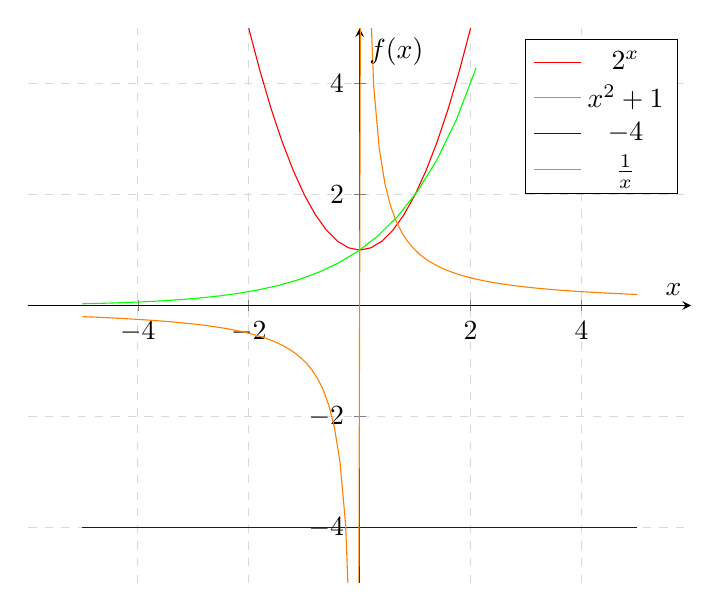
\begin{tikzpicture}
%%%
\begin{axis}[
    axis lines = left,
    xlabel = \(x\),
    ylabel = {\(f(x)\)},
    grid=major, % Display a grid
    grid style={dashed,gray!30}, % Set the
    ymin = -5,
    ymax =  5,
    xmin = -5,
    xmax =  5,
    axis equal,
    axis x line=middle,
    axis y line=middle,
]
%Below the red parabola is defined
\addplot [
    domain=-2:2, 
    samples=21,
    color=red,
]
{x^2 + 1};

%Here the green exp function
\addplot [
    domain=-5:2.1, 
    samples=21,
    color=green,
    ]
    {2^x};
\addlegendentry{\(2^x\)}


\addlegendentry{\(x^2 + 1\)}
%Here the blue constant function
\addplot [
    domain=-5:5, 
    samples=100, 
    color=blue,
    ]
    {-4};
\addlegendentry{\(-4\)}

%Here the blue constant function
\addplot [
    domain=-5:5, 
    samples=100, 
    color=orange,
    ]
    {1/x};
\addlegendentry{\(\frac{1}{x}\)}

\end{axis}
%%%
\end{tikzpicture}
\end{document}